\subsection{Types d'aphasie}

La définition qu'on a donnée de l'aphasie s'applique à une multitude de troubles  
qui touchent différents aspects de la communication~\cite[p. 135, 136]{Hallowell_2017}.
De ce fait, une classification des aphasies a été établie sur la base de leurs effets.

Plus spécifiquement, on classe une aphasie selon si elle touche l'une des trois tâches suivantes :
parler couramment, comprendre le langage et répéter la parole. 
Cela donne lieu aux huit classes qu'on voit sur la Figure~\ref{fig:aphasia-tree}.
On note  bien que cette classification n'est pas complète, l'aphasie primaire progressive par exemple n'y est pas.
Cependant, elle reste utile pour étudier les types d'aphasie qui y sont présents.


\begin{figure}[htb]
    \begin{center}
        \resizebox{\textwidth}{!}{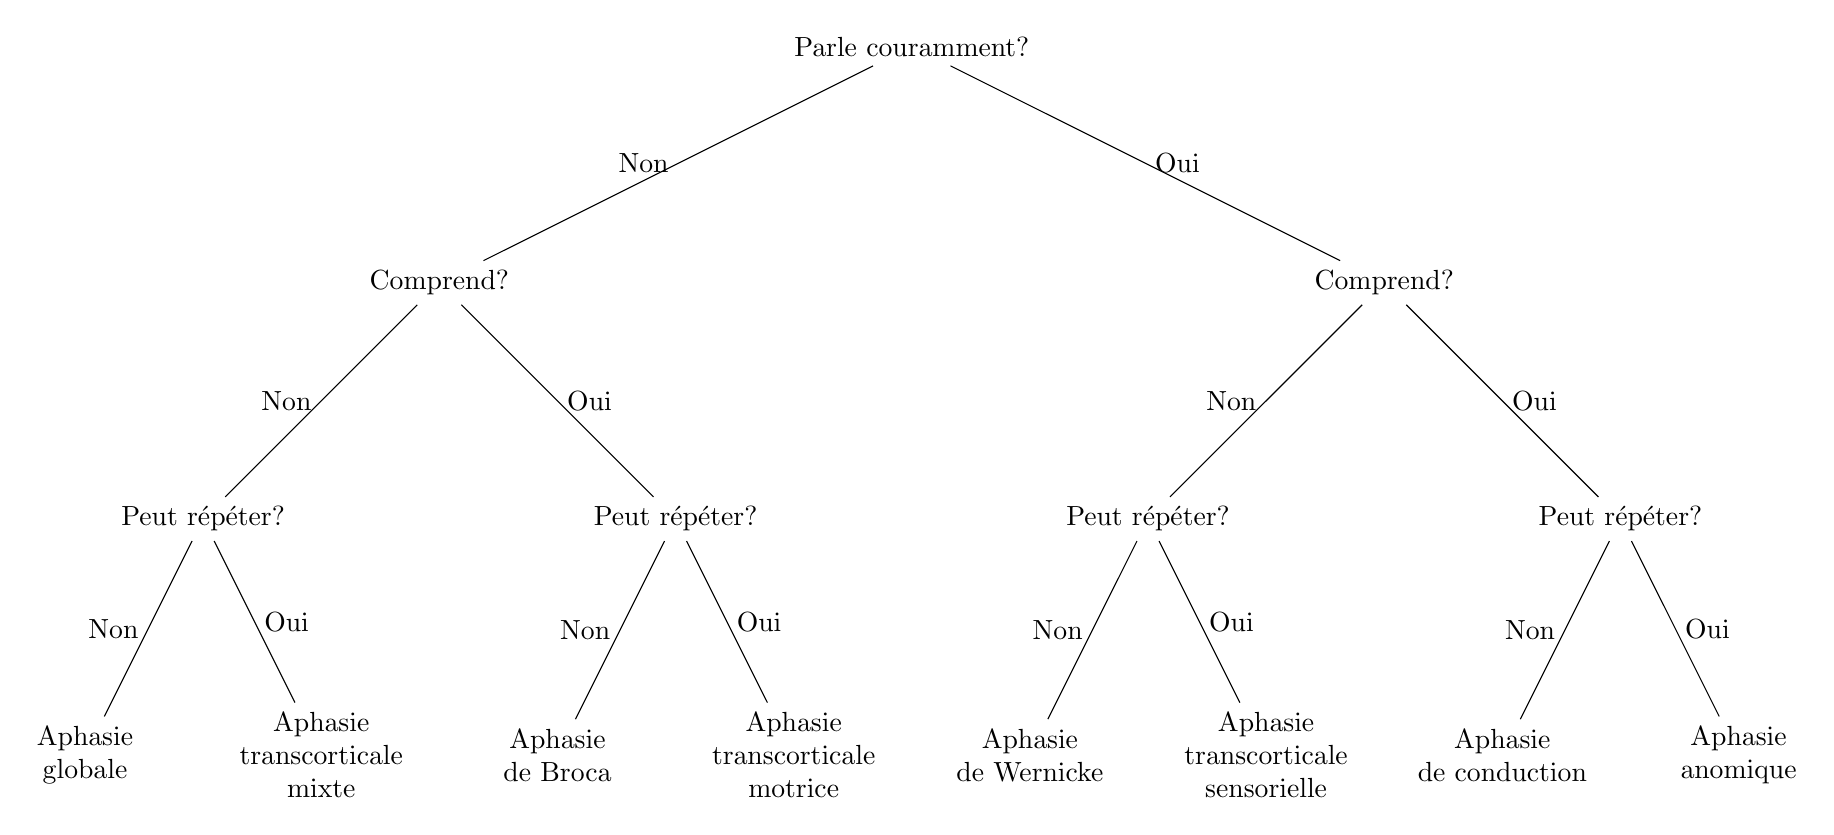
\begin{tikzpicture}
    [level distance=3cm,
    level 1/.style={sibling distance=12cm},
    level 2/.style={sibling distance=6cm},
    level 3/.style={sibling distance=3cm}
    ]
    \tikzstyle{bag} = [align=center]
    \tikzset{every tree node/.style={align=center,anchor=north}}
    % \tikzset{level distance=2cm, sibling distance=5cm}
    \node (Root)  {Parle couramment?}
        child {
            node {Comprend?} 
            child {
                node {Peut répéter?}
                child {node[bag] {Aphasie\\globale} edge from parent node[left] {Non }} 
                child {node[bag] {Aphasie\\transcorticale\\mixte} edge from parent node[right] {Oui }} 
                edge from parent node[left] {Non}   
            }
            child {
                node {Peut répéter?}
                child {node[bag] {Aphasie\\de Broca} edge from parent node[left] {Non }} 
                child {node[bag] {Aphasie\\transcorticale\\motrice} edge from parent node[right] {Oui }} 
                edge from parent node[right] {Oui}   
            } 
            edge from parent node[left] {Non} 
        }
        child {
            node {Comprend?} 
            child {
                node {Peut répéter?}
                child {node[bag] {Aphasie\\de Wernicke} edge from parent node[left] {Non }} 
                child {node[bag] {Aphasie\\transcorticale\\sensorielle} edge from parent node[right] {Oui }} 
                edge from parent node[left] {Non}   
            }
            child {
                node {Peut répéter?}
                child {node[bag] {Aphasie\\de conduction} edge from parent node[left] {Non }} 
                child {node[bag] {Aphasie\\anomique} edge from parent node[right] {Oui }} 
                edge from parent node[right] {Oui}   
            } 
            edge from parent node[right] {Oui} 
        };
    
    \end{tikzpicture}}
    \end{center}
    \caption[Classification de certains types d'aphasie]
    {Classification de certains types d'aphasie~\cite{Sreedharan_2018}}
    \label{fig:aphasia-tree}
\end{figure}

Dans cette étude, nous nous intéressons principalement à l'aphasie de Broca.
Il s'agit d'une aphasie expressive, 
c--à--d qui touche la capacité d'articuler sa pensée dans le langage et de le répéter, 
mais pas à celle de le comprendre (Voire la Figure~\ref{fig:aphasia-tree}).